\begin{frame}
  \frametitle{iCAP Goal and Obstacles}
  \begin{columns}
    \column[t]{5cm}
    \begin{figure}
      \centering
      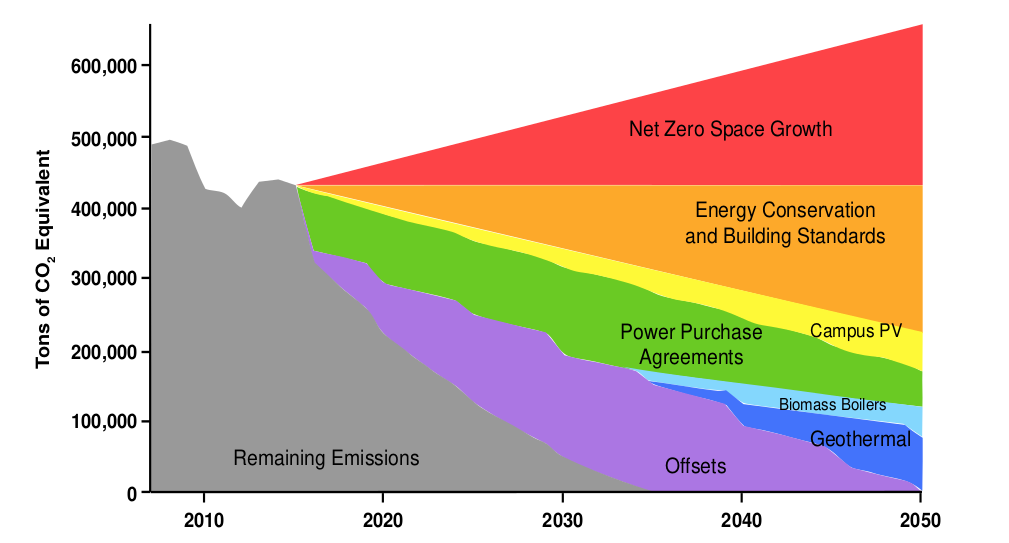
\includegraphics[width=\textwidth]{icap_uiucemissions.png}
      \caption{Shows projected CO$_2$ emissions for UIUC \cite{isee_illinois_2015}. Offsets include shutdown of the Blue Waters Supercomputer.}
      \label{fig:co2projections}
    \end{figure}

    \column[t]{5cm}
    \textbf{Goal}:\\
    Carbon neutrality by 2050 or sooner.\\
    \vspace{1cm}
    \textbf{Obstacles}:\\
    \begin{enumerate}
      \item Requires \textit{zero net space growth}.
      \item Campus depends on a system of steam tunnels for heating.
      \item and more...
    \end{enumerate}
  \end{columns}
\end{frame}

\subsection{Need for Nuclear}
\begin{frame}
  \frametitle{The Nuclear Option}
  \begin{columns}
    \vspace{0.25cm}
    \column[t]{5cm}
      \textbf{Nuclear energy...}
      \vspace{0.25cm}
      \begin{enumerate}
        \item ...produces almost no carbon emissions \cite{intergovernmental_panel_on_climate_change_climate_2014}.
        \item ...can produce high-temperature steam.
        \item ...requires little physical space$^*$.
      \end{enumerate}
      \vspace{3cm}
      *compared to solar and wind.
    \column[t]{5cm}
    \begin{figure}
      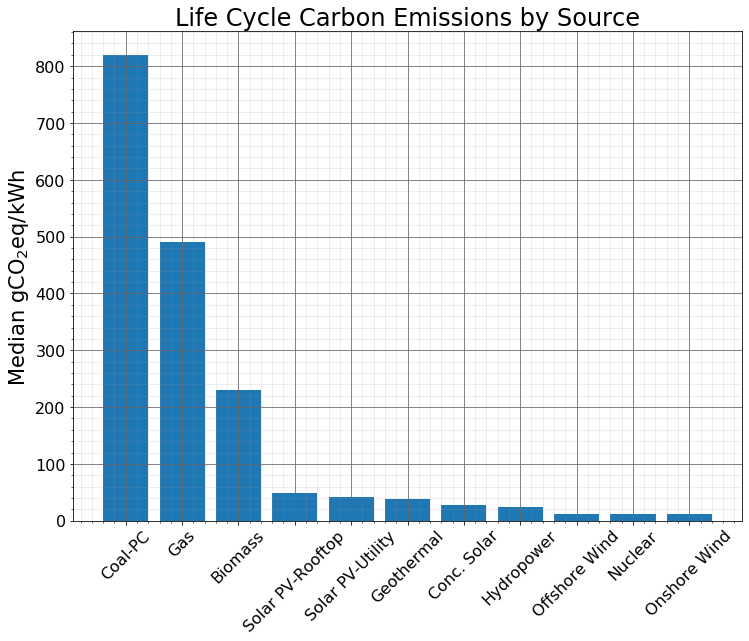
\includegraphics[width=\textwidth]{co2emissions_source.png}
      \caption{Lifetime carbon-equivalent emissions by energy source from IPCC findings \cite{intergovernmental_panel_on_climate_change_climate_2014}.}
      \label{fig:co2source}
    \end{figure}
  \end{columns}
\end{frame}

\subsection{Framing the Question}
\begin{frame}
  \begin{center}
    \Huge{\textbf{What is the optimal size for a nuclear reactor on the UIUC grid?}}
  \end{center}
\end{frame}
